\chapter{Anwendungsfall: Jitter-Analyse von Software-generierten MIDI-Clock Signalen}
\label{ch:Anwendungsfall}
Als Beispiel für ein zeitkritisches Signal sollen im Folgenden mehrere MIDI-Clock Signale mit dem Event-Recorder untersucht werden, und dabei der allgemeine Ablauf einer Event-Aufnahme und der nachfolgenden Analyse geschildert werden.
Das MIDI-Clock Signal wird in den untersuchten Fällen software-basiert (auf einem normalen Anwender-System) generiert, deswegen ist von einer messbaren zeitlichen Fluktuation (``Jitter'') auszugehen. Das heißt die Clock-Signale treten nicht exakt zum erwarteten Zeitpunkt sondern leicht zeitlich verfrüht oder verspätetet auf.\\
\acrshort{MIDI} ist ein 1983 spezifizierter Standard für den Austausch von Steuerinformationen zwischen elektronischen Musikinstrumenten und wird trotz einiger signifikanter Limitierungen seit über 35 Jahren nahezu unverändert für praktisch alle elektronischen Musikinstrumente als Standardschnittstelle verwendet. 
%Die wohl bedeutenste Limitierung ist die Verwendung von 7-bit-Werten für Parameter wie zum Beispiel den Notenwert, Anschlagstärke oder von Control-Change-Werten (also eine Beschränkung auf den Wertebereich von 0 -127).\\
MIDI bietet mit der ``MIDI-Clock'' eine Möglichkeit mehrere Geräte zeitlich zu synchronisieren. So könnte zum Beispiel ein Synthesizer mit der Musiksoftware auf einem PC synchronisiert werden, um tempo-abhängige Arpeggios\footnote{Ein Akkord bei dem die einzelnen Töne nicht gleichzeitig, sondern zeitversetzt nacheinander gespielt oder ausgelöst werden} zu spielen.\\
Dabei verwendet MIDI zur Datenübertragung das gleiche Protokoll wie ein \acrshort{UART} bei einer Übertragungsgeschwindigkeit von 31250 Bit/s (vgl. \cite{wiki:MIDI}). Die meisten MIDI-Nachrichten setzen sich aus einem Statusbyte und zwei darauf folgenden Datenbytes zusammen, für die MIDI-Clock werden allerdings nur einzelne Bytes versendet. \\
Zuerst wird ein Start-Byte (0xFA) übertragen, dann wird -- abhängig vom Tempo -- 24 mal pro Viertelnote ein ``Clock-Tick'' (0xF8) gesendet, und abschließend ein Stopp-Bit (0xFC) (siehe \cite{wiki:MIDI_clock}). \\     
\clearpage
Eine einfache Implementierung in Python mithilfe des {\tt python-rtmidi}-Moduls könnte folgendermaßen aussehen:
\begin{minted}{python}
# MIDI CLOCK TEMPO (beats per minute)
BPM = 80
# define clock messages
clock_start = [0xFA]
clock_tick  = [0xF8]
clock_stop  = [0xFC]
[...]
    # calculate clock period
    clock_period = 60 / (BPM * 24)

    # send start byte 
    midiout.send_message(clock_start)

    # run
    while (True):
        midiout.send_message(clock_tick)
        time.sleep(clock_period)

\end{minted}

\section{Test-Setup: USB-Midi mit Teensy LC}
  
Um das MIDI-Signal auswerten zu können wird ein Mikrocontroller (``Teensy LC'') verwendet, der per USB an einen PC angeschlossen werden kann, und über die USB-Schnittstelle ein MIDI-Gerät simuliert.  Das heißt am PC wird eine virtuelle MIDI-Schnittstelle erzeugt, und alle ankommenden MIDI-Daten werden direkt zum Mikrocontroller übertragen. Der Mikrocontroller wartet auf das Start-Byte einer MIDI-Clock und setzt einen GPIO-Pin auf ``1'' um dem Event-Recorder den Anfang der Aufnahme zu signalisieren. 
Danach wird bei jedem empfangenen Clock-Tick ein zweiter GPIO-Pin kurz auf ``1'' gesetzt und anschließend wieder auf ``0''. Dies soll beim Event-Recorder als Event erkannt werden. Beim Empfangen des Stopp-Bytes wird der erste GPIO-Pin auf ``0'' gesetzt und die Aufnahme wird beendet.\\
Der Teensy-Mikrocontroller kann mit der Arduino-IDE programmiert werden und es steht eine MIDI-Bibliothek zur Verfügung, was eine kurze und unkomplizierte Umsetzung erlaubt:
\begin{minted}{c}
[...]
// midi clock start handler (0xFA)
void onStart() {
  digitalWrite(0, HIGH);
}

// midi clock tick handler (0xF8) 
void onClock() {
    digitalWrite(1, HIGH);
    digitalWrite(1, LOW);
}

// midi clock stop handler (0xFC)
void onStop() {
  digitalWrite(0, LOW);
}

void setup() {
  // pin setup
  [...]
  // register midi handlers
  usbMIDI.setHandleStart(onStart);
  usbMIDI.setHandleStop(onStop);
  usbMIDI.setHandleClock(onClock);
}

void loop() {
  usbMIDI.read();
}
\end{minted}

\section{Einrichten des Projekts}
\label{ch:Anwendungsfall:sec:Einrichten}

Die vollständige Einrichtung des Raspberry Pi Zero W soll hier aus Platzgründen nicht beschrieben werden (es steht aber eine detailliertere Anleitung im Projekt-Wiki zur Verfügung).
Der grundsätzliche Ablauf ist wie folgt:
\begin{enumerate}

\item Download, Kompilieren und Installation der {\tt IceStorm}-Toolchain auf dem Anwender-PC (Linux-System)

\begin{minted}{bash}
# siehe http://www.clifford.at/icestorm/#install
\end{minted}

\item Download, Kompilieren und Installation der RISC-V Toolchain auf dem Anwender-PC

\begin{minted}{bash}
git clone git@github.com:cliffordwolf/picorv32.git
cd picorv32
make download-tools
make -j\$(nproc) build-tools
\end{minted}

Das Kompilieren der RISC-V {\tt gcc}-Toolchain kann je nach Rechenleistung mehrere Stunden dauern.

\item Download des Git-Projekts auf dem Anwender-PC (Linux-System)

\begin{minted}{bash}
cd ..
git clone https://github.com/dm7h/icozsoc.git
\end{minted}


\item Einrichten der SSH-Verbindung zum Raspberry Pi Zero W 

\begin{minted}[breaklines]{bash}
# siehe zum Beispiel: https://www.raspberrypi.org/documentation/remote-access/ssh/passwordless.md
# Exportieren des SSH-Hosts, z.B. pi@zero oder pi@192.168.1.43:
export SSH_RASPI=pi@zero
# eine SSH-Verbindung sollte dann ohne Passwort-Abfrage möglich sein:
ssh $SSH_RASPI $
\end{minted}

\item Download, Kompilieren und Installation des {\tt icozctl} Git-Projekts auf dem Raspberry Pi\\ 
Zur Installation des {\tt icozctl}-Tools wird auf dem Raspberry Pi folgendes ausgeführt:
\begin{minted}{bash}
git clone https://github.com/dm7h/icozctl
cd icozctl
sudo make install
\end{minted}

\item Generieren und Programmieren des Bitfiles mithilfe des zur Verfügung gestellten {\tt Makefiles}\\
Wenn {\tt icozctl} erfolgreich auf dem Raspberry Pi installiert wurde, kann auf dem Anwender-PC das FPGA-Bitstream und die 
IcoSoc-Anwendung kompiliert und via Raspberry Pi auf die Hardware geflasht werden:
\begin{minted}{bash}
cd ../icosoc/examples/event-recorder/
make prog_flash
\end{minted}

 
\end{enumerate}

\section{Konfiguration der Event-Trigger}
\label{ch:Anwendungsfall:sec:Event-Trigger}

Um die Events zu konfigurieren wird zunächst per SSH auf das Raspberry Pi gewechselt.  
Im Ordner des {\tt icozctl}-Tools befindet sich die Event-Konfigurationsdatei {\tt config.yml}.
Für die Aufnahme wird nicht zwangsläufig eine Event-Erkennung benötigt, es kann aber aber trotzdem ein Start-, Stopp- und Clock-Event definiert werden um unnötige Aufnahmedaten zu minimieren:

\begin{lstlisting}[language=yaml]
# event configuration
events: 
  - start:
          trigger: u
          funcion: start

  - stop:
          trigger: d
          function: stop

  - clk_up:
          trigger: 1u

  - clk_down:
          trigger: 1d
\end{lstlisting}

\section{Vorbereiten der Hardware}
\label{ch:Anwendungsfall:sec:Vorbereitung}

Bevor die Event-Aufnahme gestartet werden kann müssen die am Mikrocontroller konfigurierten Ausgangs-Pins mit den Eingangs-Pins des Event-Recorders verbunden werden.
In unserem Fall wird der Ausgang ``0'' und ``1'' des Teensy LC mit den Eingängen ``0'' und ``1'' am Pmod-Header P3 des IceZero-Boards verbunden und zusätzlich wird mit einen ``GND''-Pin eine Masse-Verbindung hergestellt. Siehe zur Pin-Belegung auch den Anhang ``\nameref{sec:pmod_pins}''. 

\section{Durchführen der Event-Aufnahme}
\label{ch:Anwendungsfall:sec:Durchführung}

Die Auswertung soll zu Anschauungszwecken das \acrshort{VCD}-Dateiformat verwenden.
Die Aufnahme kann dann mit folgendem Befehl gestartet werden:
\begin{minted}{bash}
icozctl -c config.yml -o midi_clock.vcd
\end{minted}

Das Programm wartet nun auf Eingangsdaten, die zum Beispiel durch das Starten der in Python implementieren Midi-Clock oder durch ein Musik-Programm geliefert werden können.
Die Aufnahme kann zu jedem Zeitpunkt durch die Tastenkombination Strg+c beendet werden.
Alternativ kann {\tt icozctl} auch mit der Option ``-N'' gestartet werden, um die Aufnahme nach einer festgelegten Anzahl von Samples zu beenden. 
\begin{minted}{bash}
icozctl -N 512 -c config.yml -o midi_clock.vcd
\end{minted}
Das Ergebnis der Aufnahme kann dann zum Beispiel mit dem Programm {\tt gtkwave}\cite{web:gtkwave} oder mit {\tt pulseview}\cite{web:pulseview} grafisch dargestellt und überprüft werden:
\begin{figure}[H]
	\centering
	\captionsetup{justification=centering,margin=2cm}
		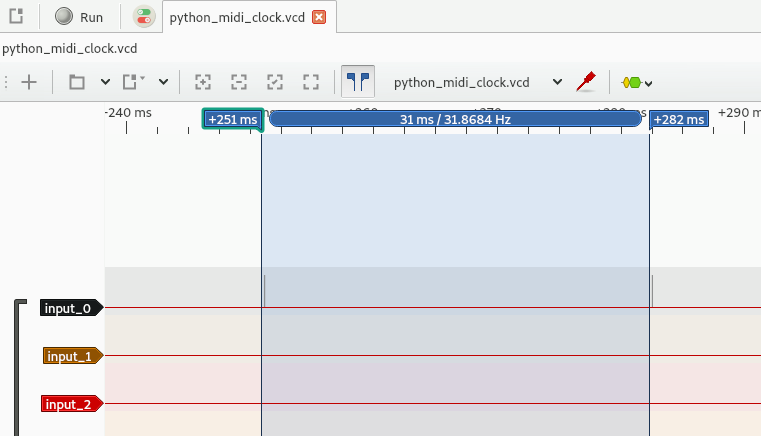
\includegraphics[width=\textwidth]{../figures/midi_clock_pulseview.png}
		\caption[Darstellung eines aufgenommenen Midi-Clock-Signals mit Pulseview]{Darstellung eines aufgenommenen Midi-Clock-Signals mit Pulseview (Quelle: Pulseview-Screenshot)}
	\label{fig:ice40_pmod_pins}
\end{figure}


\section{Analyse der Ergebnisse}
\label{ch:Anwendungsfall:sec:Analyse}

Für die Analyse der Daten kann zum Beispiel ein Python-Skript verwendet werden. Um Aussagen über den Jitter des Signals machen zu können bietet sich die Generierung eines Histogramms an, bei dem auf der x-Achse die Abweichung zum erwarteten Clock-Signal und auf der y-Achse die Häufigkeit der Abweichung dargestellt wird.

Für das Einlesen der VCD-Datei wird das Python-Modul {\tt Verilog\_VCD}\cite{web:verilog_vcd} verwendet:
\begin{minted}{python}
import Verilog_VCD
vcd = Verilog_VCD.parse_vcd('midi_clock.vcd')
\end{minted}

Im VCD-Dateiformat wird jedem Signal ein Symbol als Abkürzung zugewiesen, auf die Daten des ersten Signals der Datei kann zum Beispiel mit der Abkürzung ``!'' zugegriffen werden (siehe ``\nameref{sec:pmod_pins}'' für eine Zuordnung der Signal-Abkürzungen).
Die Zeitstempel sind in der Python-Liste unter dem Index "tv" (``time value'') abrufbar. 
Der zeitliche Abstand zum jeweils vorhergehenden Event (Zeit-Delta) kann folgendermaßen berechnet werden:
 
\begin{minted}{python}
# get the first time value
last = vcd["!"]["tv"][0][0]

# calculate time deltas
deltas = []
for item in vcd["!"]["tv"][1:]: 
    deltas.append(item[0]-last)
    last = item[0]
\end{minted}

Die Daten werden in ein numpy-Array umgewandelt und es wird die Differenz zum erwarteten Zeit-Delta gebildet. 
Anschließend werden sie in eine pandas-Zeitserie konvertiert, wodurch automatisch statistisch relevante Kennwerte wie der Mittelwert und die Standardabweichung berechnet und angezeigt werden können:
 
\begin{minted}{python}
np_deltas = np.array(deltas)
expected_delta = 31250000 # expected clock period in nanoseconds
np_deltas -= expected_delta
print(deltas_series.describe())
\end{minted}

Die Ausgabe sieht zum Beispiel\footnote{Die Werte stammen von der oben beschriebenen Python-Implementierung, das Zeit-Delta wird hier in Mikrosekunden-Auflösung angezeigt} folgendermaßen aus:

\begin{minted}{c}
count                        86
mean     0 days 00:00:00.000125
std      0 days 00:00:00.000026
min      0 days 00:00:00.000053
25%      0 days 00:00:00.000109
50%      0 days 00:00:00.000117
75%      0 days 00:00:00.000131
max      0 days 00:00:00.000227

\end{minted}

Abschließend kann mithilfe der matplotlib-Bibliothek ein Histogramm in Millisekunden-Auflösung erzeugt und angezeigt werden:

\begin{minted}{python}
(deltas_series/pd.Timedelta(milliseconds = 1)).hist()
[...]
plt.show()
\end{minted}

\clearpage

\subsection{Software MIDI-Clock: Python-Implementierung}
Für die erste Messung wurde die Python-Implementierung verwendet.\
\begin{figure}[H]
	\centering
	\captionsetup{justification=centering,margin=2cm}
		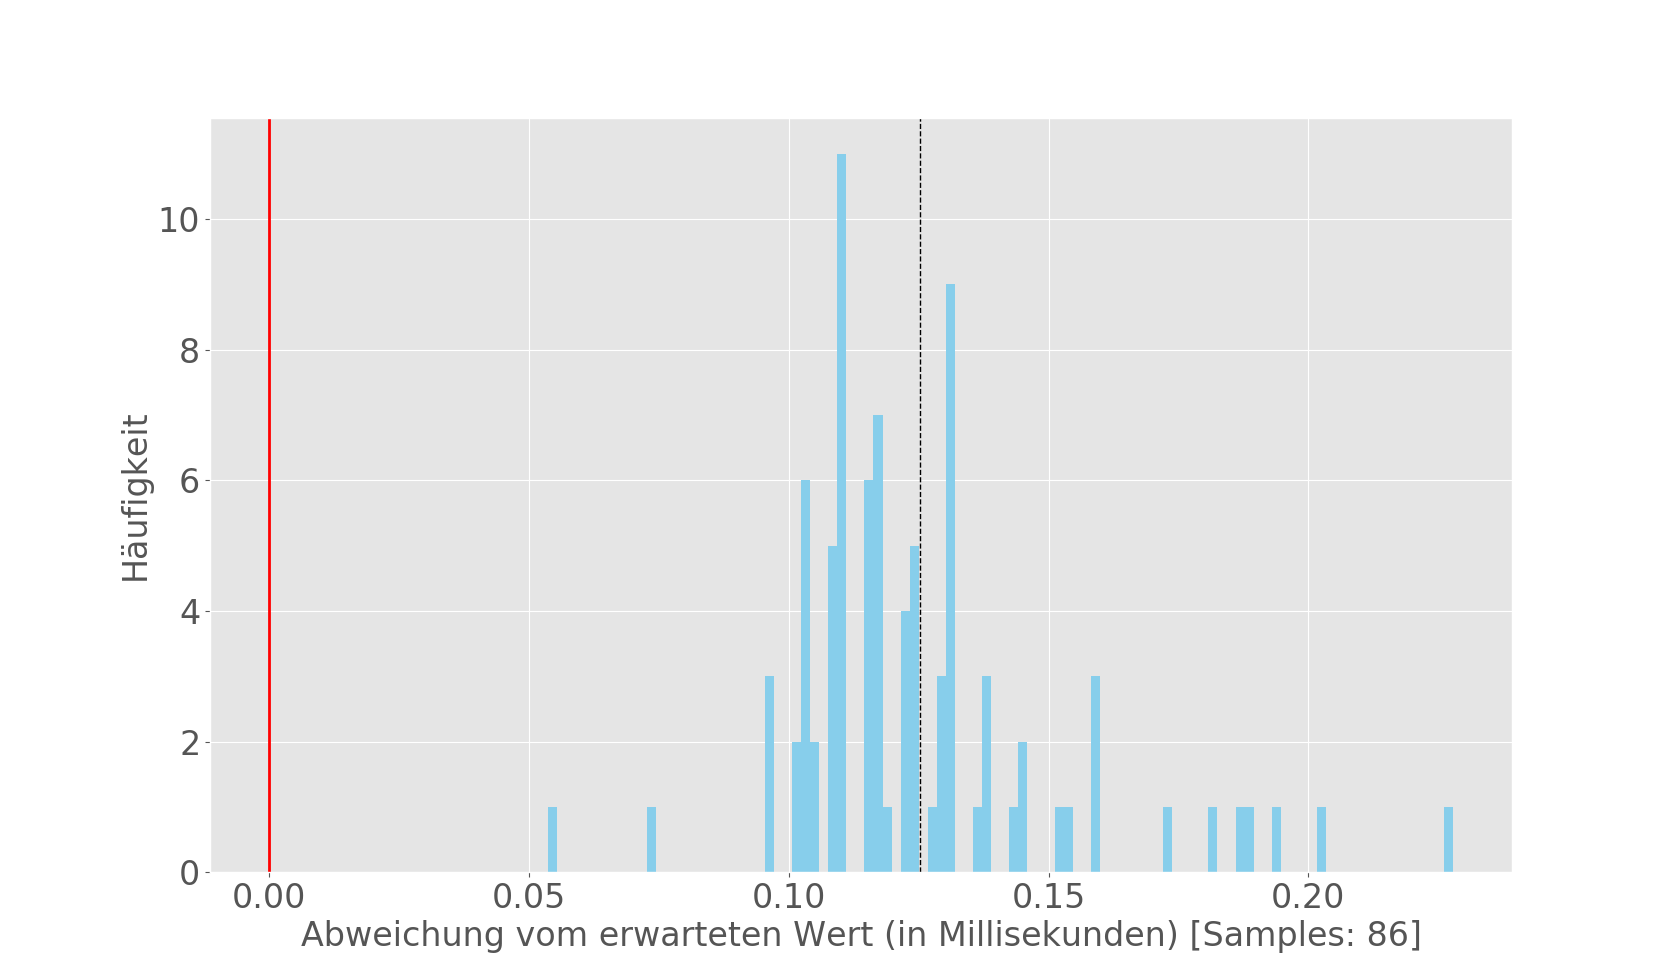
\includegraphics[width=\textwidth]{../figures/clock_python.png}
		\caption[Histogramm der Python-generierten MIDI-Clock]{Histogramm der Python-generierten MIDI-Clock}
	\label{fig:ice40_pmod_pins}
\end{figure}
Die erwartete Abweichung (0) ist mit der roten Linie markiert, der Mittelwert mit der gestrichelten schwarzen Linie.\\
Auffällig ist hier vor allem dass die MIDI-Clock langsamer läuft als erwartet, da eine konstante positive Abweichung von ca. 0,125 Millisekunden vorliegt. Dies lässt sich dadurch erklären, dass bei jedem Ausführen des {\tt midiout.sendmessage(clock\_tick)}-Befehls zusätzlich zur berechneten Clock-Periode Zeit verbraucht wird. Der Jitter liegt bei circa 0,2 Millisekunden und ist damit vergleichsweise niedrig.


\subsection{Software MIDI-Clock: Renoise und Reaper}

Anschließend wurde die MIDI-Clock von den Musikprogrammen Renoise und Reaper aufgenommen\footnote{Es wurden (von den Vorlieben des Autors abgesehen) keine besonderen Auswahlkriterien verfolgt, beide Programme haben eine kostenlose Demo-Version mit der die Funktionalität geprüft werden kann}.

\begin{figure}[H]
	\centering
	\captionsetup{justification=centering,margin=2cm}
		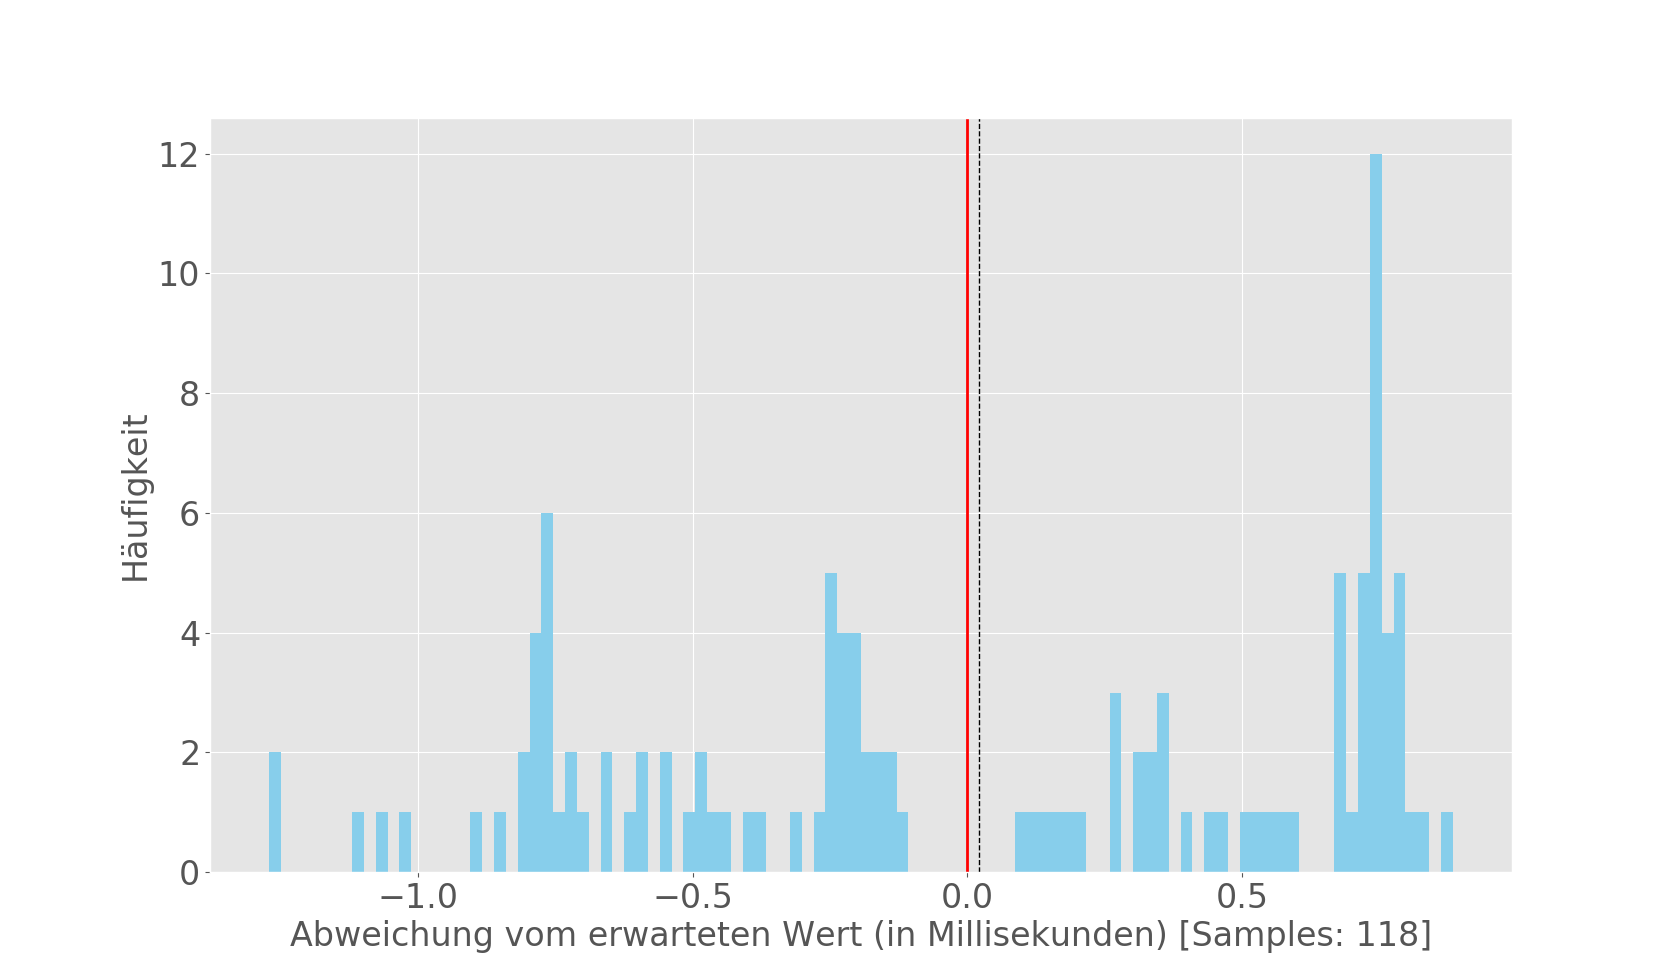
\includegraphics[width=\textwidth]{../figures/clock_renoise.png}
		\caption[Histogramm der MIDI-Clock des Musik-Programms Renoise]{Histogramm der MIDI-Clock des Musik-Programms Renoise}
	\label{fig:ice40_pmod_pins}
\end{figure}

Bei der MIDI-Clock von Renoise zeigt sich ein Jitter von fast 2 Millisekunden -- ein eher schlechter Wert bei dem sogar hörbare Konsequenzen auftreten könnten.
Die Wahrnehmung von zeitlichen Verzögerungen ist stark vom betroffenen Audio-Material abhängig. Bei einem zeitlichen Versatz von zwei identischen Signalen kann das zweite Signal bereits ab 0,6 Millisekunden als Reflexion wahrgenommen werden, und beeinflusst dementsprechend den Charakter des Audio-Materials. Zu einem differenzierbaren Echo-Effekt kommt es erst bei Zeitverschiebungen von 20 Millisekunden oder mehr (vgl. \cite[S.~29]{ma:falke}).   


\begin{figure}[H]
	\centering
	\captionsetup{justification=centering,margin=2cm}
		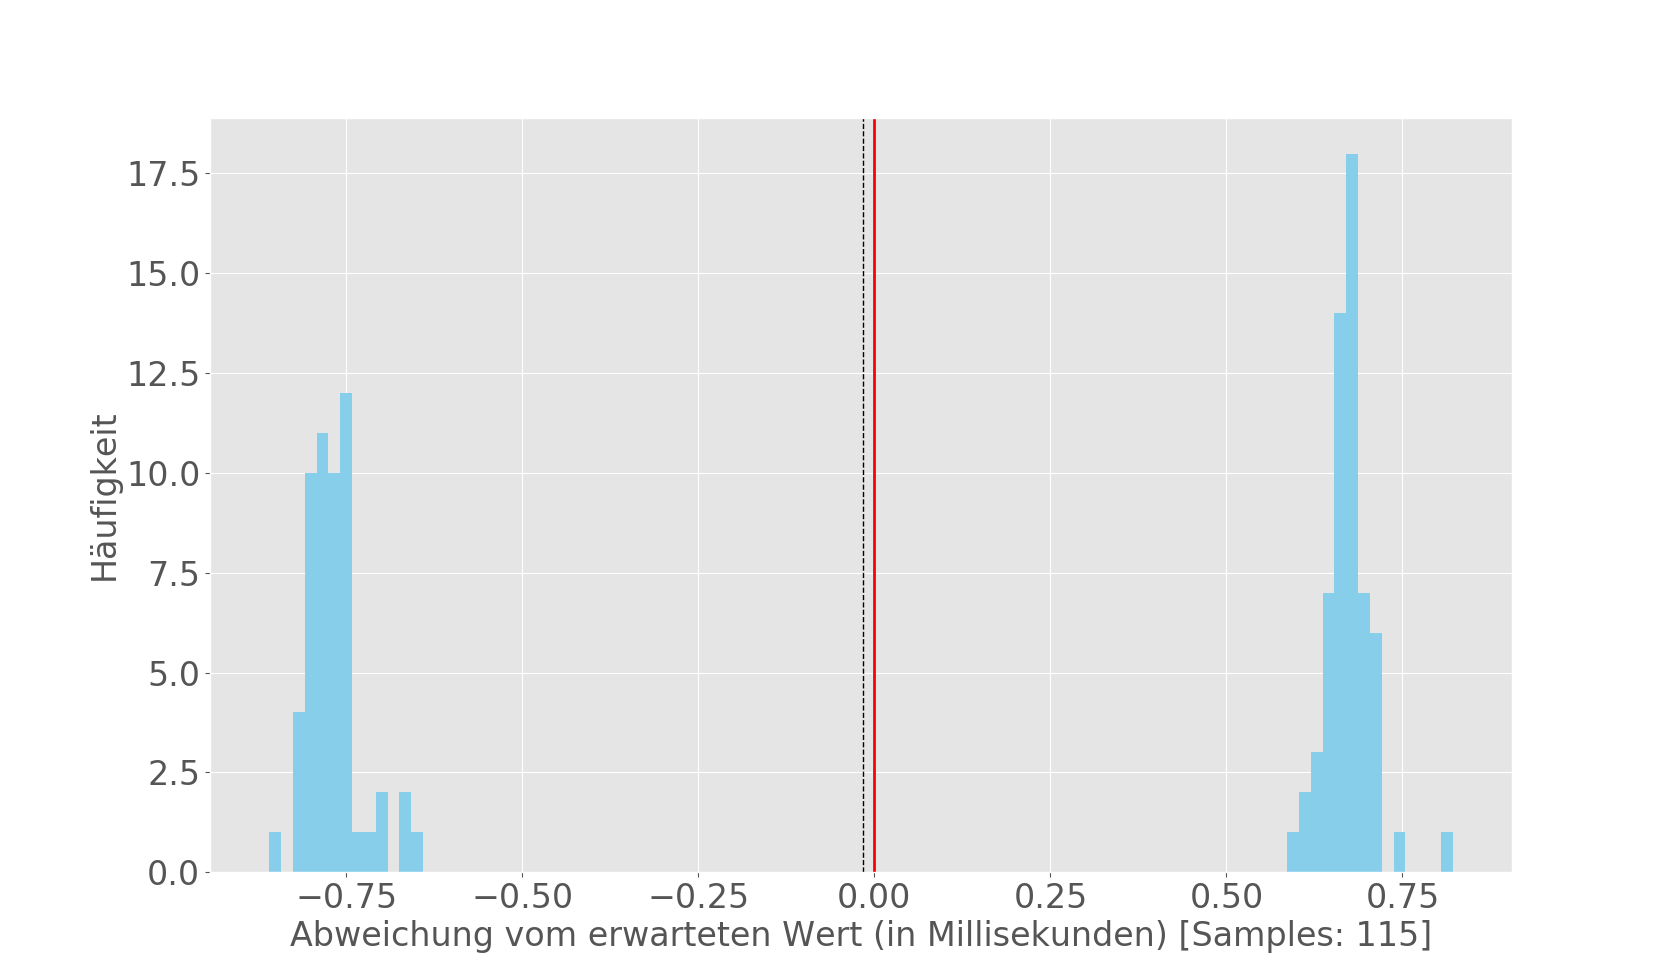
\includegraphics[width=\textwidth]{../figures/clock_reaper.png}
		\caption[Histogramm der MIDI-Clock des Musik-Programms Reaper]{Histogramm der MIDI-Clock des Musik-Programms Reaper}
	\label{fig:ice40_pmod_pins}
\end{figure}

Bei der MIDI-Clock von Reaper fällt der Jitter mit circa 1,5 Millisekunden etwas geringer aus und zeigt eine starke ausgeprägte bimodale Verteilung. Auch dies ist -- inbesondere im Vergleich zur ``naiven'' Python-Implementierung -- ein eher schlechter Wert.

\subsection{Hardware MIDI-Clock: Midipal}
Abschließend wurde noch die auf einem ATMega328p-Mikrocontroller basierende Hardware-MIDI-Clock des ``MIDIpal''\footnote{Das ``MIDIpal'' ist ein Open-Source-Hardwareprodukt der Firma Mutable Instruments, das allerdings nicht mehr kommerziell angeboten wird (siehe \cite{web:midipal})} getestet. Das Clock-Signal wurde über den MIDI-Eingang einer RME Digiface PCI-Soundkarte erfasst und mit einer Software-Loopback auf das virtuelle MIDI-Interface des Teensy LC geroutet.

\begin{figure}[H]
	\centering
	\captionsetup{justification=centering,margin=2cm}
		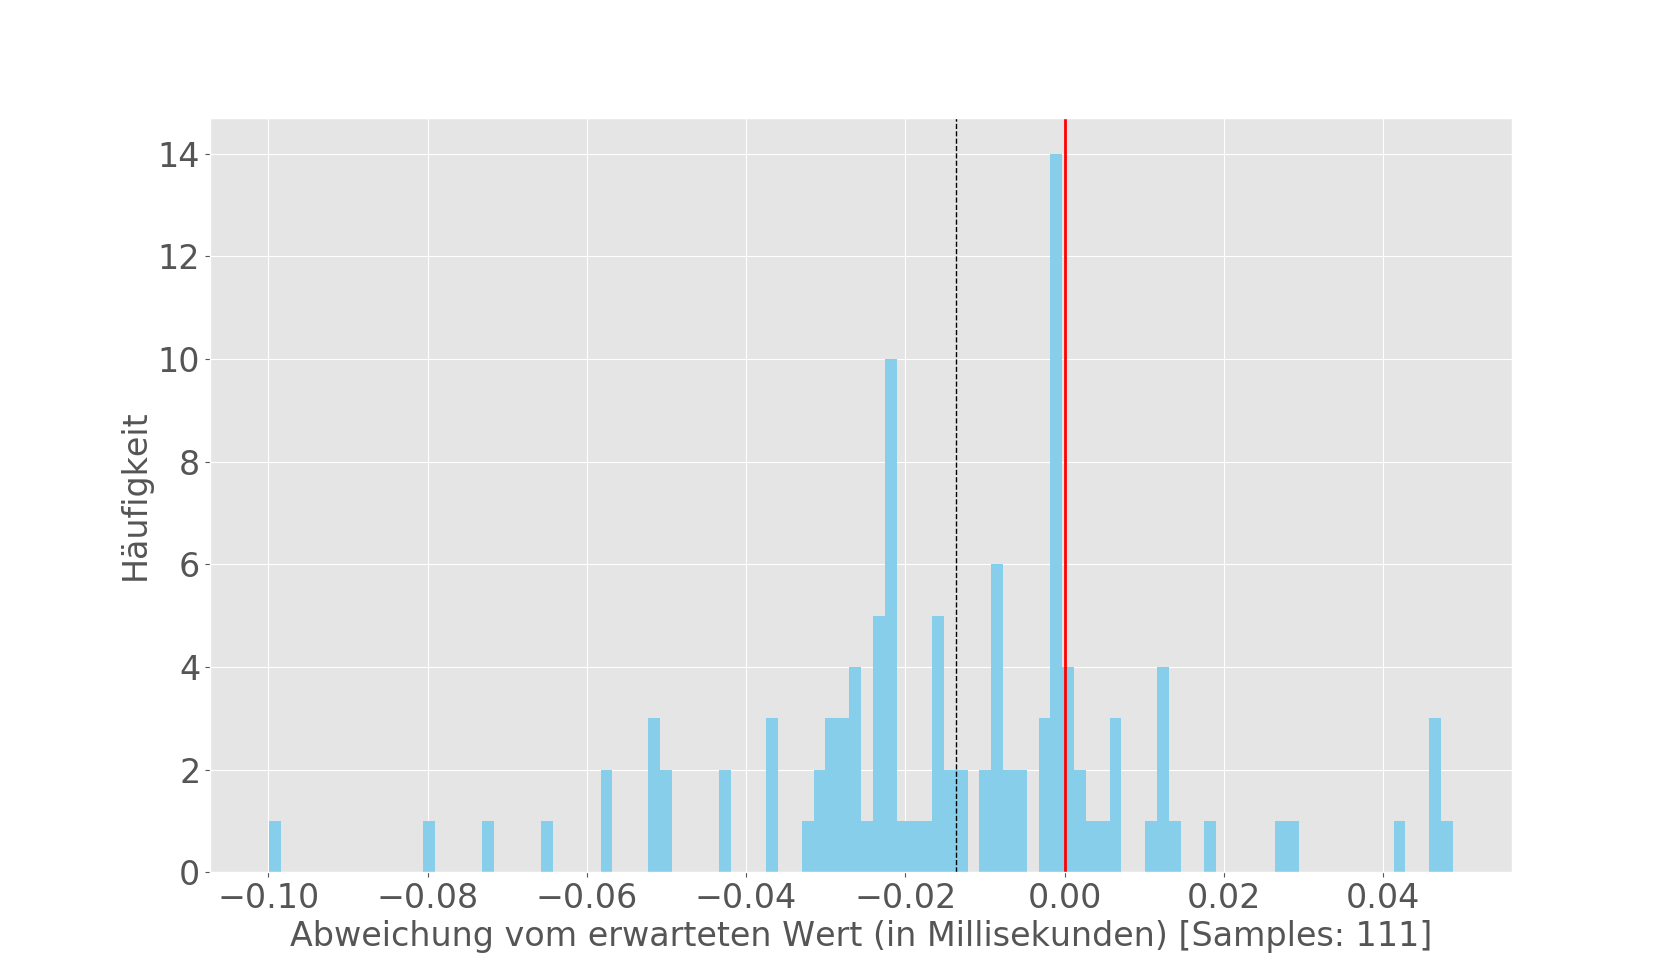
\includegraphics[width=\textwidth]{../figures/clock_midipal.png}
		\caption[Histogramm einer Mikrocontroller-generierten Hardware-MIDI-Clock]{Histogramm einer Mikrocontroller-generierten Hardware-MIDI-Clock (Mutable Instruments MidiPal)}
	\label{fig:ice40_pmod_pins}
\end{figure}

Die Messung liefert ein deutlich stabileres Ergebnis mit einem Jitter von circa 0,15 Millisekunden. Es zeigt sich, dass die Mikrocontroller-basierte Lösung den beiden Software-Produkten in Hinblick auf die Stabilität des Clock-Signals überlegen ist.

Zu allen Messungen ist anzumerken, dass der Teensy-Mikrocontroller (der mit einer Taktfrequenz von 40 Mhz läuft) einen -- nicht näher bestimmten -- verfälschenden Einfluss auf das Endergebnis hat. Alle Messungen wurden wiederholt mit variierenden Samplezahlen durchgeführt, und die beschriebenen Charakteristika sind ohne nennenswerte Abweichungen reproduzierbar. Dementsprechend kann davon ausgegangen werden, dass die vom Teensy verursachte Messverfälschung für die Analyse vernachlässigbar ist.


